\chapter{Parallelisierung der kritischen Abschnitte}

Um einer optimalen Leistung nahezukommen, wurde bei der Implementierung ein iterativer Ansatz gewählt. Hierzu wurden zuerst die Möglichkeiten der Parallelisierung und anschließend die der Optimierung in Python betrachtet und aufeinander aufbauend implementiert. 

\section{Parallelisierung}

\subsection{Parallelisierung der Verarbeitung einzelner Bildpaare mittels MPI}

Da die zu bearbeitenden Bildpaare voneinander unabhängig sind, lassen sich diese trivial parallelisieren. Der Vorteil dieses Ansatzes liegt besonders in seiner simplen Implementierung und erwarteten linearen Skalierung begründet. Dieser Ansatz bringt allerdings auch Nachteile mit sich: Einige \gls{MPI}-Implementierungen erlauben das Erstellen neuer Threads nur, wenn dies beim Installieren der Bibliotheken angegeben wird \cite{OMPI17} und es ist nur eine schwache Skalierung zu erwarten. Sofern kein Multithreading innerhalb von \gls{MPI} möglich ist, limitiert die Anzahl der Bildpaare die Parallelisierungsmöglichkeit stark. In der auf dem GitHub-Branch \textit{mpi} verfügbaren Implementierung dieses Ansatzes wird pro Bildpaar  primär ein Kern genutzt \cite{CBS18}. Die Initialisierung wird dabei vom Masterkern übernommen, dessen Aufgabe es auch ist, die Bildpaare auf weitere Kerne zu verteilen. Zum Schluss werden die Ergebnisse wieder beim Masterkern gesammelt und gespeichert.

Die parallele Bearbeitung eines Bildpaares wird, wie bereits zuvor, von der joblib-Bibliothek übernommen, welche die Nutzung von Multithreading in Python ermöglicht. Hierbei wurde nicht sichergestellt, dass unter Verwendung mehrerer Rechenknoten die Bildpaare gleichmäßig auf diese verteilt wurden. 

\subsection{Parallelisierung innerhalb der Verarbeitung einzelner Bildpaare mittels MPI}

Eine sinnvolle Erweiterung zur oben beschriebenen Methode ist das Ersetzen der genutzten Mul\-ti\-threa\-ding-Bibliothek mittels MPI, sodass selbst die Berechnung eines einzelnen Bildpaares über Rechnergrenzen hinweg möglich ist. In diesem Zuge wurde auch die Fehlerkorrektur am Ende des Speckle-Trackings parallelisiert, indem die zu korrigierenden Bildausschnitte auf mehrere Kerne verteilt wurden. Zusätzlich erleichtert diese Implementierung den Einsatz eines Tracing-Programmes, wie SCORE-P \cite{KRM+12}. Dies war aufgrund der unterliegenden multiprocessing-Bibliothek zuvor nicht trivial möglich. Ein hoher Speed-Up wird insbesondere für wenige zu korrigierende Bildausschnitte nicht erwartet. 

Im Konkreten werden die Bildpaare auf \gls{CPU}-Kern-Gruppen verteilt, welche durch gleichmäßiges Aufteilen der verfügbaren \gls{CPU}-Kerne erstellt werden. Einer dieser Kerne innerhalb der Gruppe agiert hierbei als Hauptkern und ist dafür verantwortlich, das Bildpaar zu verarbeiten, wobei dieser Aufgaben mittels eines \gls{MPI}-Kommunikators an die anderen Rechenkerne der Gruppe verteilen kann. Die Aufgabe des Masterkerns ist es, die Bildpaare gleichmäßig auf die Gruppen zu verteilen. Dies ist beispielhaft in der Abbildung \ref{fig:parallel_concept} gezeigt. Sollten mehr Bildpaare als Rechenkerne vorhanden sein, werden mehrere Bildpaare von einem Kern hintereinander verarbeitet. 

Die Programmierschnittstelle wurde so entworfen, dass die Verteilung der Bildpaare auf die Kerne und das Parallelisieren innerhalb dieser für den Programmierer transparent geschieht. Hierbei gibt der Nutzer lediglich drei Funktionszeiger an: einen für die Initialisierungsfunktion, einen für die Hauptverarbeitungsroutine und einen für die Endfunktion. Die Initialisierungsfunktion generiert hierbei zwei Listen: eine mit globalen Parametern, die später an alle Hauptkerne gesendet wird, und eine mit lokalen Parametern, die auf die einzelnen \gls{CPU}-Kern-Gruppen verteilt werden. Die so verteilten Daten werden der Hauptverarbeitungsroutine übergeben, welche die Daten parallel verarbeitet und das Ergebnis zurückgibt. Dieses wird anschließend auf dem Masterkern gesammelt und der Endfunktion übergeben. 

Innerhalb der Hauptverarbeitungsroutine bietet eine Schnittstelle auf die \gls{CPU}-Kern-Gruppe eine weitere Parallelisierungsmöglichkeit. Diese Schnittstelle wurde hierbei ähnlich zur joblib-Implementierung entworfen. Auch hier werden wieder ein Funktionszeiger und lokale sowie globale Parameter entgegengenommen, die analog zu der oben beschriebenen Methode in der Gruppe verteilt werden. Eine exemplarische Implementierung eines Programmes, welches jedes Element in einer Matrix mit einem bestimmten Wert multiplizieren und anschließend einen weiteren aufaddieren soll, ist in Listing \ref{lst:dist_api} gezeigt. Ein mittels der joblib implementiertes, funktional äquivalentes Programm ist in Listing \ref{lst:joblib} dargestellt. Die äquivalente Ausgabe der beiden Programme ist in Listing \ref{lst:ausgabe} dokumentiert. Die Implementierung dieses Ansatzes ist auf dem GitHub-Branch \textit{mpi-advanced} zu finden \cite{CBS18}.

\begin{lstlisting}[caption={Parallelisierung mittels der in \gls{MPI} implementierten Version},label={lst:dist_api}]
from distributor import Distributor
def $\textit{initFn}$():
	$\textit{global\_args}$ = (1, 2)
	$\textit{local\_args}$ = [[1, 5], [2, 6], [3, 7], [4, 8]]
	return ($\textit{global\_args}$, $\textit{local\_args}$)
def $\textit{addFn}$($\textit{global\_args}$, $\textit{local\_args}$):
	($\textit{multiply}$, $\textit{add}$) = $\textit{global\_args}$
	return $\textit{local\_args}$ * $\textit{multiply}$ + $\textit{add}$
def $\textit{mainFn}$($\textit{global\_args}$, $\textit{local\_args}$, $\textit{dist}$):
	return $\textit{dist}$.parallel($\textit{addFn}$, $\textit{global\_args}$, $\textit{local\_args}$)
def $\textit{exitFn}$($\textit{global\_args}$, $\textit{result}$):
	print("The result is", $\textit{result}$)
	return 0
$\textit{dist}$ = Distributor($\textit{initFn}$, $\textit{mainFn}$, $\textit{exitFn}$)
\end{lstlisting}

\begin{lstlisting}[caption={Parallelisierung mittels der joblib-Bibliothek},label={lst:joblib}]
from joblib import Parallel, delayed
import multiprocessing
def $\textit{addFn}$($\textit{array}$, $\textit{multiply}$, $\textit{add}$):
	$\textit{result}$ = []
	for $\textit{element}$ in $\textit{array}$:
		$\textit{result}$ += [$\textit{element}$ * $\textit{multiply}$ + $\textit{add}$]
	return $\textit{result}$
$\textit{matrix}$ = [[1, 5], [2, 6], [3, 7], [4, 8]]
$\textit{multiply}$ = 1
$\textit{add}$ = 2
$\textit{n\_jobs}$ = len($\textit{matrix}$)
$\textit{result}$ = Parallel()(delayed($\textit{addFn}$)($\textit{matrix}$[$\textit{k}$], $\textit{multiply}$, $\textit{add}$) for $\textit{k}$ in range($\textit{n\_jobs}$))
print("The result is", $\textit{result}$)
\end{lstlisting}

\begin{lstlisting}[language=C, caption={Ausgabe der Programme}, label={lst:ausgabe}]
The result is [[3, 7], [4, 8], [5, 9], [6, 10]]
\end{lstlisting}

\begin{center}
	\begin{figure}[htbp]
		\centering
		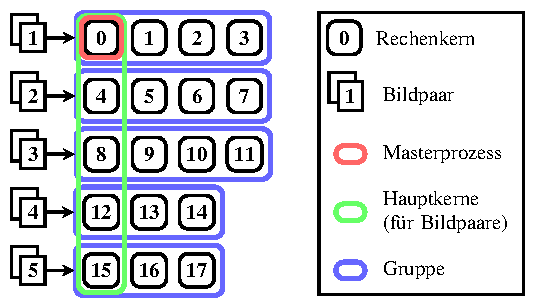
\includegraphics[width=0.5\textwidth]{pdf/parallel}
		\caption[Verteilung]{Verteilung von fünf Bildpaaren auf 18 Rechenknoten}
		\label{fig:parallel_concept}
	\end{figure}
\end{center}

\section{Optimierung der Performance-Engpässe in Python}

Wie in Abbildung \ref{fig:perc_slow} zu sehen ist, werden über 95\% der Rechenzeit in den fünf langsamsten Funktionen verbracht. Unter diesen ist insbesondere die \texttt{nxcorr\_disp()}-Funktion, welche komplett in Python implementiert ist. Um die Leistung solcher Funktionen zu verbessern, werden im Folgenden Methoden zur Optimierung des bestehenden Codes betrachtet -- mit besonderem Augenmerk auf der Beschleunigung der langsamsten Funktionen. 

\subsection{Nutzen bereits optimierter Funktionen}

Einige Teile des Codes können durch bereits in Python oder einer optimierten Bibliothek enthaltenen Funktion ersetzt werden, womit der Interpretieraufwand erheblich reduziert wird. Dies gehört damit zu einer der grundlegenden Optimierungsmöglichkeiten. Zusätzlich dazu enthalten diese Funktionen bereits Plattform-spezifische Optimierungen. In der Funktion \texttt{nxcorr\_disp()} lassen sich Code-Abschnitte mit diesem Verbesserungspotential finden. Das Listing \ref{lst:max2} zeigt den Codeausschnitt aus dieser Funktion zum Ermitteln eines Maximums einer Matrix in reinem Python-Code, wobei die äußeren Zeilen und Spalten vernachlässigt werden. Listing \ref{lst:max2_fast} zeigt einen funktional äquivalenten Code unter Nutzung von bereits optimierten Funktionen. \texttt{lengthX} und \texttt{lengthY} geben hier die Dimensionen der Eingabematrix \texttt{nxcorr} an. 

\begin{lstlisting}[caption={Finden des Maximums einer Matrix}, label={lst:max2}]
for $\textit{i}$ in range(1, $\textit{lengthY}$ - 1):
	for $\textit{j}$ in range(1, $\textit{lengthX}$ - 1):
		if($\textit{nxcorr}$[$\textit{i}$, $\textit{j}$] > $\textit{maxValue}$):
			$\textit{maxValue}$ = $\textit{nxcorr}$[$\textit{i}$, $\textit{j}$]
			$\textit{maxI}$ = $\textit{i}$
			$\textit{maxJ}$ = $\textit{j}$
\end{lstlisting}

\begin{lstlisting}[caption={Finden des Maximums einer Matrix mittels NumPy und OpenCV}, label={lst:max2_fast}]
$\textit{nxcorr\_small}$ = $\textit{nxcorr}$[1:-1, 1:-1]
(_, $\textit{maxValue}$, _, ($\textit{maxJ}$, $\textit{maxI}$)) = cv2.minMaxLoc($\textit{nxcorr\_small}$)
$\textit{maxI}$ += 1
$\textit{maxJ}$ += 1
\end{lstlisting}

\begin{sloppypar}
	Des Weiteren befindet sich in der \texttt{nxcorr\_disp()}-Funktion die Berechnung des Signal-Rausch-Verhältnisses (gezeigt im Listing \ref{lst:snr_calc}), was allerdings im weiteren Verlauf des Programmes nicht wieder verwendet wird und deshalb entfernt werden kann. 
\end{sloppypar}

\begin{lstlisting}[caption={Berechnung des Signal-Rausch-Verhältnisses}, label={lst:snr_calc}]
$\textit{avg}$ = 0.0
$\textit{count}$ = 0
for $\textit{i}$ in range($\textit{lengthY}$):
	for $\textit{j}$ in range($\textit{lengthX}$):
		if(($\textit{i}$ is not $\textit{maxI}$) and ($\textit{j}$ is not $\textit{maxJ}$)):
			$\textit{avg}$ = $\textit{avg}$ + abs($\textit{nxcorr}$[$\textit{i}$,$\textit{j}$])
			$\textit{count}$ = $\textit{count}$ + 1
$\textit{avg}$ = $\textit{avg}$ / float()$\textit{count}$)
$\textit{SNr}$ = $\textit{maxValue}$ / $\textit{avg}$
\end{lstlisting}

Nach dem Anwenden dieser Änderungen befindet sich keine in Python implementierte Schleife mehr in der Funktion. Angesichts der hohen Aufrufzahl von \texttt{nxcorr\_disp()} und dem Entfernen großer Codeanteile ist ein hoher Beschleunigungsfaktor zu erwarten. 

Zum Schluss wurde die Evaluierung des zu verwendenden Korrelationsalgorithmus in der \texttt{norm\_xcorr()}-Funktion, gezeigt in Listing \ref{lst:eval}, durch eine direkte Variable (gezeigt in Listing \ref{lst:var}) ersetzt. Eine Version des Codes mit allen hier vorgeschlagenen Optimierungen ist auf dem Branch \texttt{intrinsics} des GitHub-Repositorys zu finden \cite{CBS18}. 

\begin{lstlisting}[caption={Evaluierung der Korellationsmethode}, label={lst:eval}]
def $\textit{norm\_xcorr}$($\textit{template}$, $\textit{searchArea}$, $\textit{method}$='cv2.TM_CCOEFF_NORMED'):
	$\textit{meth}$ = eval($\textit{method}$)
	#...
\end{lstlisting}

\begin{lstlisting}[caption={Übergabe der Korellationsmethode als Variable}, label={lst:var}]
def $\textit{norm\_xcorr}$($\textit{template}$, $\textit{searchArea}$, $\textit{method}$=cv2.TM_CCOEFF_NORMED):
	$\textit{meth}$ = $\textit{method}$
	#...
\end{lstlisting}

\subsection{Kompilieren}

Eine weitere Möglichkeit der Minimierung des Python-Engpasses ist die Übersetzung des Python-Codes in nativen Maschinencode. Die möglichen Ansätze hierbei reichen von der Übersetzung des gesamten Programmes über die Übersetzung einzelner Funktionen, die in Python dann als Modul geladen werden können, bis hin zur Nutzung eines \gls{JIT}-Compilers, welcher annotierte Funktionen bei dessen ersten Aufruf in nativen Maschinencode übersetzt. 

\subsubsection{Gesamtes Programm}

Die einfachste Möglichkeit der Übersetzung ist es, das gesamte Programm in Maschinencode zu übersetzten. Hierzu kann die Bibliothek cython \cite{BBD+17} genutzt werden, welche Python-Code in C übersetzt, was anschließend in Maschinencode übersetzt werden kann. Hierzu wurde nur die Datei \textit{waveFront.py} unübersetzt gelassen, da diese keine rechenaufwendigen Funktionen enthält und diese nur aus anderen Dateien, insbesondere der \textit{func.py} aufruft. Die benötigten Installationsdateien sind auch dem GitHub-Branch \textit{compiled} verfügbar \cite{CBS18}. 

\subsubsection{Einzelne Funktionen}

\paragraph{numba}

numba ist eine Optimierungsbibliothek für Python, welche unter anderem die Möglichkeit bietet, Funktionen \gls{JIT} zu übersetzen sowie CUDA\footnote{\url{https://developer.nvidia.com/cuda-zone}} und OpenCL\footnote{\url{https://www.khronos.org/opencl}} zu nutzen \cite{LPS15}. Funktionen können zur \gls{JIT}-Übersetzung mittels der Annotation \texttt{@jit} markiert werden. Sobald während der Ausführung diese Funktion erreicht wird, übersetzt numba den Code in eine Intermediate-Repräsentation, welche anschließend von LLVM weiter in Maschinencode übersetzt wird. Beim nächsten Aufruf wird die annotierte Funktion in einer Liste aller übersetzten Funktionen gesucht und es wird sofort der Maschinencode der Funktion verwendet. Ein permanentes Speichern des Übersetzungsergebnisses ist mittels der Annotiation \texttt{@jit(cached = True)} möglich. Auf dem \texttt{numba}-Branch befindet sich eine Version des Codes, in dem diese Annotationen genutzt werden \cite{CBS18}. Annotiert wurden hierbei Funktionen zur Auswahl der \gls{ROI} innerhalb der \texttt{cpCorr()}-Funktion und die \texttt{nxcorr\_disp()}-Funktion.

\paragraph{Cython}

Eine weitere weitaus mächtigere Methode zur Übersetzung einzelner Funktionen bietet die Cython-Bibliothek, welche bereits genutzt wurde, um das gesamte Programm zu übersetzen. Diese führt die Möglichkeit der Typisierung ein und lässt die direkte Einbindung von C zu. In der auf dem GitHub-Branch \textit{cython} verfügbaren Version wurde Cython genutzt, um die Funktionen \texttt{norm\_xcorr()} (siehe Listing \ref{lst:cython_nxc}) und \texttt{nxcorr\_disp()} (siehe Listing \ref{lst:cython_nxd}) zu übersetzen \cite{CBS18}. Hierbei wurden alle Variablen mit Typen versehen und es wurde die von Cython bereitgestellte Schnittstelle zu NumPy genutzt. Auf dem Branch \textit{compiled-advanced} wurde die Übersetzung des gesamten Programmes mit den hier optimierten Funktionen zusammengeführt \cite{CBS18}. 

\begin{lstlisting}[caption={Die in Cython optimierte Funktion norm\_xcorr()}, label={lst:cython_nxc}]
def $\textit{norm\_xcorr}$(np.ndarray[float, ndim=2] $\textit{template}$, np.ndarray[float, ndim=2] $\textit{searchArea}$, int $\textit{method}$ = cv2.TM_CCOEFF_NORMED):
	cdef $\textbf{double}$ $\textit{minVal}$ = 0.0, $\textit{maxVal}$ = 0.0
	cdef tuple $\textit{minLoc}$, $\textit{maxLoc}$
	cdef np.ndarray[float, ndim=2] $\textit{corr}$ = cv2.matchTemplate($\textit{searchArea}$, $\textit{template}$, $\textit{method}$)
	$\textit{minVal}$, $\textit{maxVal}$, $\textit{minLoc}$, $\textit{maxLoc}$ = cv2.minMaxLoc($\textit{corr}$)
	return $\textit{corr}$, $\textit{minVal}$, $\textit{maxVal}$, $\textit{minLoc}$, $\textit{maxLoc}$
\end{lstlisting}

\begin{lstlisting}[caption={Die in Cython optimierte Funktion nxcorr\_disp()}, label={lst:cython_nxd}]
def $\textit{nxcorr\_disp}$(np.ndarray[float, ndim=2] $\textit{nxcorr}$):
	cdef int $\textit{lengthY}$ = $\textit{nxcorr}$.shape[0]
	cdef int $\textit{lengthX}$ = $\textit{nxcorr}$.shape[1]
	# find maximum
	$\textit{nxcorr\_small}$ = $\textit{nxcorr}$[1:-1, 1:-1]
	cdef int $\textit{maxI}$, $\textit{maxJ}$
	(_, _, _, ($\textit{maxJ}$, $\textit{maxI}$)) = cv2.minMaxLoc($\textit{nxcorr\_small}$)
	$\textit{maxI}$ += 1
	$\textit{maxJ}$ += 1
	# calculate offset using gaussian subpixel interpolation
	cdef $\textbf{double}$ $\textit{dy}$ = ($\textit{nxcorr}$[$\textit{max}$I + 1, $\textit{maxJ}$] - $\textit{nxcorr}$[$\textit{maxI}$ - 1, $\textit{maxJ}$]) / 2.0
	cdef $\textbf{double}$ $\textit{dyy}$ = $\textit{nxcorr}$[$\textit{maxI}$ + 1, $\textit{maxJ}$] + $\textit{nxcorr}$[$\textit{maxI}$ - 1, $\textit{maxJ}$] - 2.0 * $\textit{nxcorr}$[$\textit{maxI}$, $\textit{maxJ}$]
	cdef $\textbf{double}$ $\textit{dx}$ = ($\textit{nxcorr}$[$\textit{maxI}$, $\textit{maxJ}$ + 1] - $\textit{nxcorr}$[$\textit{maxI}$, $\textit{maxJ}$ - 1]) / 2.0
	cdef $\textbf{double}$ $\textit{dxx}$ = ($\textit{nxcorr}$[$\textit{maxI}$, $\textit{maxJ}$ + 1] + $\textit{nxcorr}$[$\textit{maxI}$, $\textit{maxJ}$ - 1] - 2.0 * $\textit{nxcorr}$[$\textit{maxI}$, $\textit{maxJ}$])
	cdef $\textbf{double}$ $\textit{dxy}$ = ($\textit{nxcorr}$[$\textit{maxI}$ + 1, $\textit{maxJ}$ + 1] - $\textit{nxcorr}$[$\textit{maxI}$ + 1, $\textit{maxJ}$ - 1] - $\textit{nxcorr}$[$\textit{maxI}$ - 1, $\textit{maxJ}$ + 1] + $\textit{nxcorr}$[$\textit{maxI}$ - 1, $\textit{maxJ}$ - 1]) / 4.0
	# calculate normalization factor
	cdef $\textbf{double}$ $\textit{det}$ = 0.0
	if(($\textit{dxx}$ * $\textit{dyy}$ - $\textit{dxy}$ * $\textit{dxy}$) != 0.0):
		$\textit{det}$ = 1.0 / ($\textit{dxx}$ * $\textit{dyy}$ - $\textit{dxy}$ * $\textit{dxy}$)
	# calculate new subpixel indices
	cdef $\textbf{double}$ $\textit{ix}$ = - ($\textit{dyy}$ * $\textit{dx}$ - $\textit{dxy}$ * $\textit{dy}$) * $\textit{det}$ + $\textit{maxJ}$ - ($\textit{lengthX}$//2)
	cdef $\textbf{double}$ $\textit{iy}$ = - ($\textit{dxx}$ * $\textit{dy}$ - $\textit{dxy}$ * $\textit{dx}$) * $\textit{det}$ + $\textit{maxI}$ - ($\textit{lengthY}$//2)
	$\textit{out}$ = []
	$\textit{out}$.append($\textit{iy}$)
	$\textit{out}$.append($\textit{ix}$)
	return $\textit{out}$
\end{lstlisting}